\section{Sistemas de controle}
    \subsection{Definição de Sistemas de Controle}
        Um sistema de controle é um método automatizado, formado pela ligação entre vários componentes, que permite manipular e gerenciar o desempenho de um determinado processo de forma a obter, em sua saída, um valor desejado de referência \cite{Livro_Ogata} e garantir sua operação em uma zona segura e estável de valores. Todo processo envolve alguma operação física, transformação ou transporte de matéria ou energia.
        
        Aplicados aos fornos de convecção forçada, os sistemas de controle garantem a operação desses dispositivos em valores estipulados de temperatura, assegurando um processo confiável e que atenda às especificações para qualidade do alimento.
        
        A resposta do sistema de controle a um determinado estímulo de entrada pode ser dividida nos períodos transitório e estacionário. A resposta transitória refere-se ao estado inicial da curva, em que o sinal varia muito rapidamente no tempo e que tende a um estado final chamado de resposta estacionária ou permanente, região em que o comportamento do sinal de saída possui pouca ou nenhuma variação com o tempo. A amplitude da saída, no regime permanente, é dita como valor final.
        
        O comportamento dos sistemas de controle descreve uma relação causal entre as grandezas de saída e de entrada, sendo, normalmente, representados por diagramas em blocos que facilitam a visualização e compreensão do seu funcionamento. Cada um desses blocos representa uma característica matemática e possui um modelo que descreve seu comportamento.
    \subsection{Modelagem matemática de sistemas de controle}
        O modelo matemático de um sistema de controle, apresentando os blocos e componentes interligados, é mostrado pelo diagrama da Figura ~\ref{fig:ModeloSistema}:
        \begin{figure}[H]
            \centering
            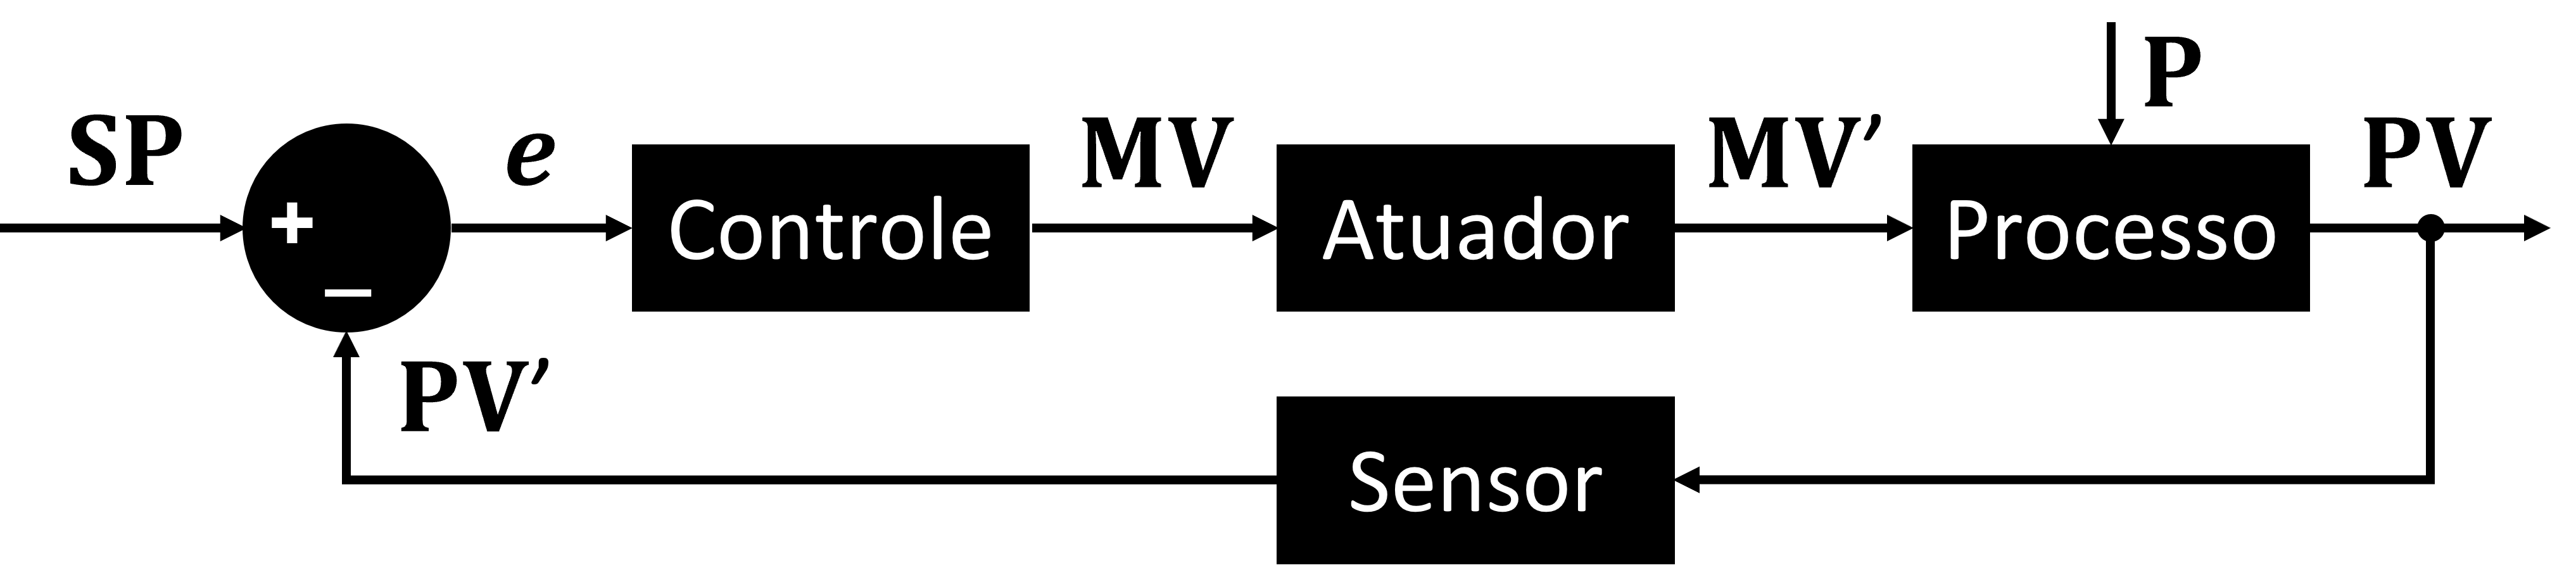
\includegraphics[width=0.48\textwidth]{Figuras/ModeloSistema.png}
            \caption{Modelagem matemática de um sistema de controle.} \label{fig:ModeloSistema}
        \end{figure}
        
        O modelo, acima, define:
        \begin{itemize}
            \item \SetPoint \ (SP) $-$ “Valor alvo” ou “referência de entrada”: define a amplitude desejada para a grandeza de saída do sistema, ou seja, é o valor de saída que o sistema deve fornecer. Aplicado ao forno de convecção forçada, o \SetPoint \ é a temperatura desejada de operação do forno; 
            \item Erro (\textit{e}): caracteriza erro atual presente no sistema, ou seja, diferença entre o valor atual do processo (temperatura do forno) e o \SetPoint;
            \item Variável manipulada (MV): representa a variável modificada pelo controle, a fim de alterar o valor da variável do processo. Na prática, os sistemas de controle não alteram, diretamente, a variável controlada. O fato é que há uma variação no comportamento do elemento atuador que garante alterações na variável controlada. Para o caso da temperatura, por exemplo, a variável manipulada apresenta-se, entre outras formas, na potência média fornecida pelo elemento gerador de calor;
            \item Perturbação (P): as perturbações tratam-se de distúrbios que, inseridos na malha de controle, causam alterações no valor da saída do sistema, aumentando, exponencialmente, o valor absoluto do erro. Tais fenômenos ocorrem por diversos fatores e, geralmente, representam um sinal de baixa frequência \cite{TCC_Controle1};
            \item Valor do processo (PV): amplitude da grandeza de saída do processo. 
        \end{itemize}
    
        O controle pode ser realizado por um Controlador Lógico Programável (CLP) ou por outros dispositivos, com o objetivo de entregar, na saída, uma amplitude igual ao valor definido no \SetPoint. Variações podem ocorrer na amplitude da grandeza de saída, em função da mudança do \SetPoint \ ou de perturbações que afetem o sistema, mas o controle é capaz de corrigir os dois efeitos, minimizando, ou anulando completamente, o erro após o período transitório. 
        
        O controle altera o estado do dispositivo atuador, a fim de modificar a grandeza variável do sistema. Analisando as características dos fornos, a geração de calor, nesses elementos, ocorre por uma resistência de aquecimento, dispositivo que gera calor ao circular uma corrente elétrica pelo condutor. Dessa forma, a resistência de aquecimento admite-se como o elemento atuador, uma vez que seu comportamento é capaz de alterar a amplitude da grandeza de saída.
        
        O valor atual da grandeza de saída do sistema é medido pelo elemento sensor. Para o caso de temperatura, os elementos sensores, geralmente, são os termopares ou termo-resistências \cite{Fundamentos_SistemasControle}, os quais podem apresentar-se de diferentes tipos, dependendo de algumas características, como, por exemplo, a temperatura de calibração.
    \subsection{Sistemas de controle em malha aberta e malha fechada}
        Os sistemas de controle, de acordo com o tipo de operação, podem ser classificados de duas formas:
    
        \begin{itemize}
            \item Controle em malha aberta: operação comumente aplicada a sistemas estáticos no tempo, nessa técnica de controle não há realimentação, ou seja, o controle atua em relação ao valor do \SetPoint, sem comparação com a amplitude da saída, conforme ilustrado na Figura ~\ref{fig:MalhaAberta}. Os sistemas de controle em malha aberta são simples e apresentam baixo custo de implementação, porém trata-se de uma técnica imprecisa de controle;
            \begin{figure}[H]
                \centering
                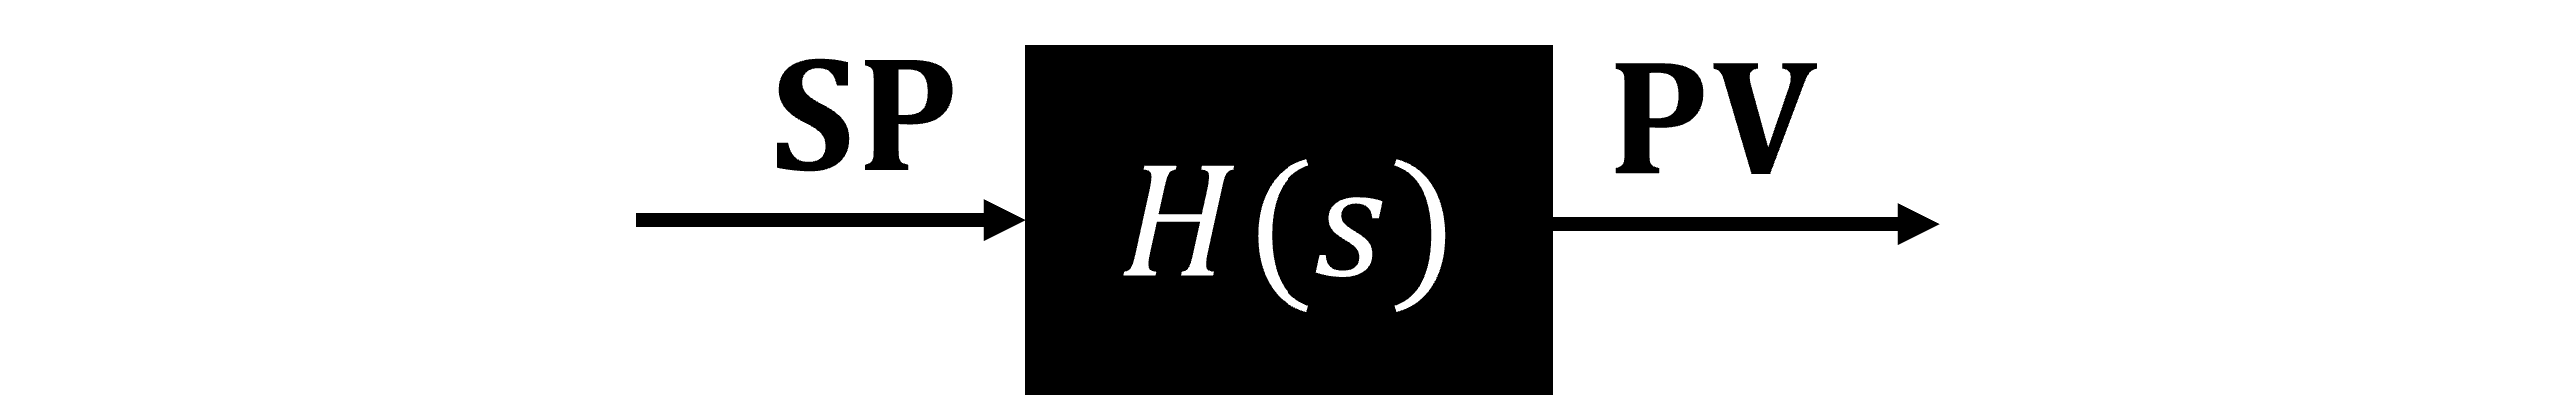
\includegraphics[width=0.35\textwidth]{Figuras/MalhaAberta.png}
                \caption{Sistema de controle em malha aberta.} \label{fig:MalhaAberta}
            \end{figure}
            
            \item Controle em malha fechada: operação comumente aplicada a sistemas dinâmicos no tempo, nessa técnica de controle há uma malha de realimentação (ou \textit{feedback}), ou seja, há uma comparação entre o valor desejado do sistema (\SetPoint) e a amplitude da saída (PV), definindo o erro atual, conforme ilustrado na Figura ~\ref{fig:MalhaFechada}, em que $C(s)$ representa o sistema de controle, $G(s)$, o processo e $H(s)$, a malha de realimentação. Nesse caso, o erro caracteriza a entrada do sistema, alterando o estado do atuador e da variável manipulada a fim de reduzir o erro absoluto a zero.
    
            \begin{figure}[H]
                \centering
                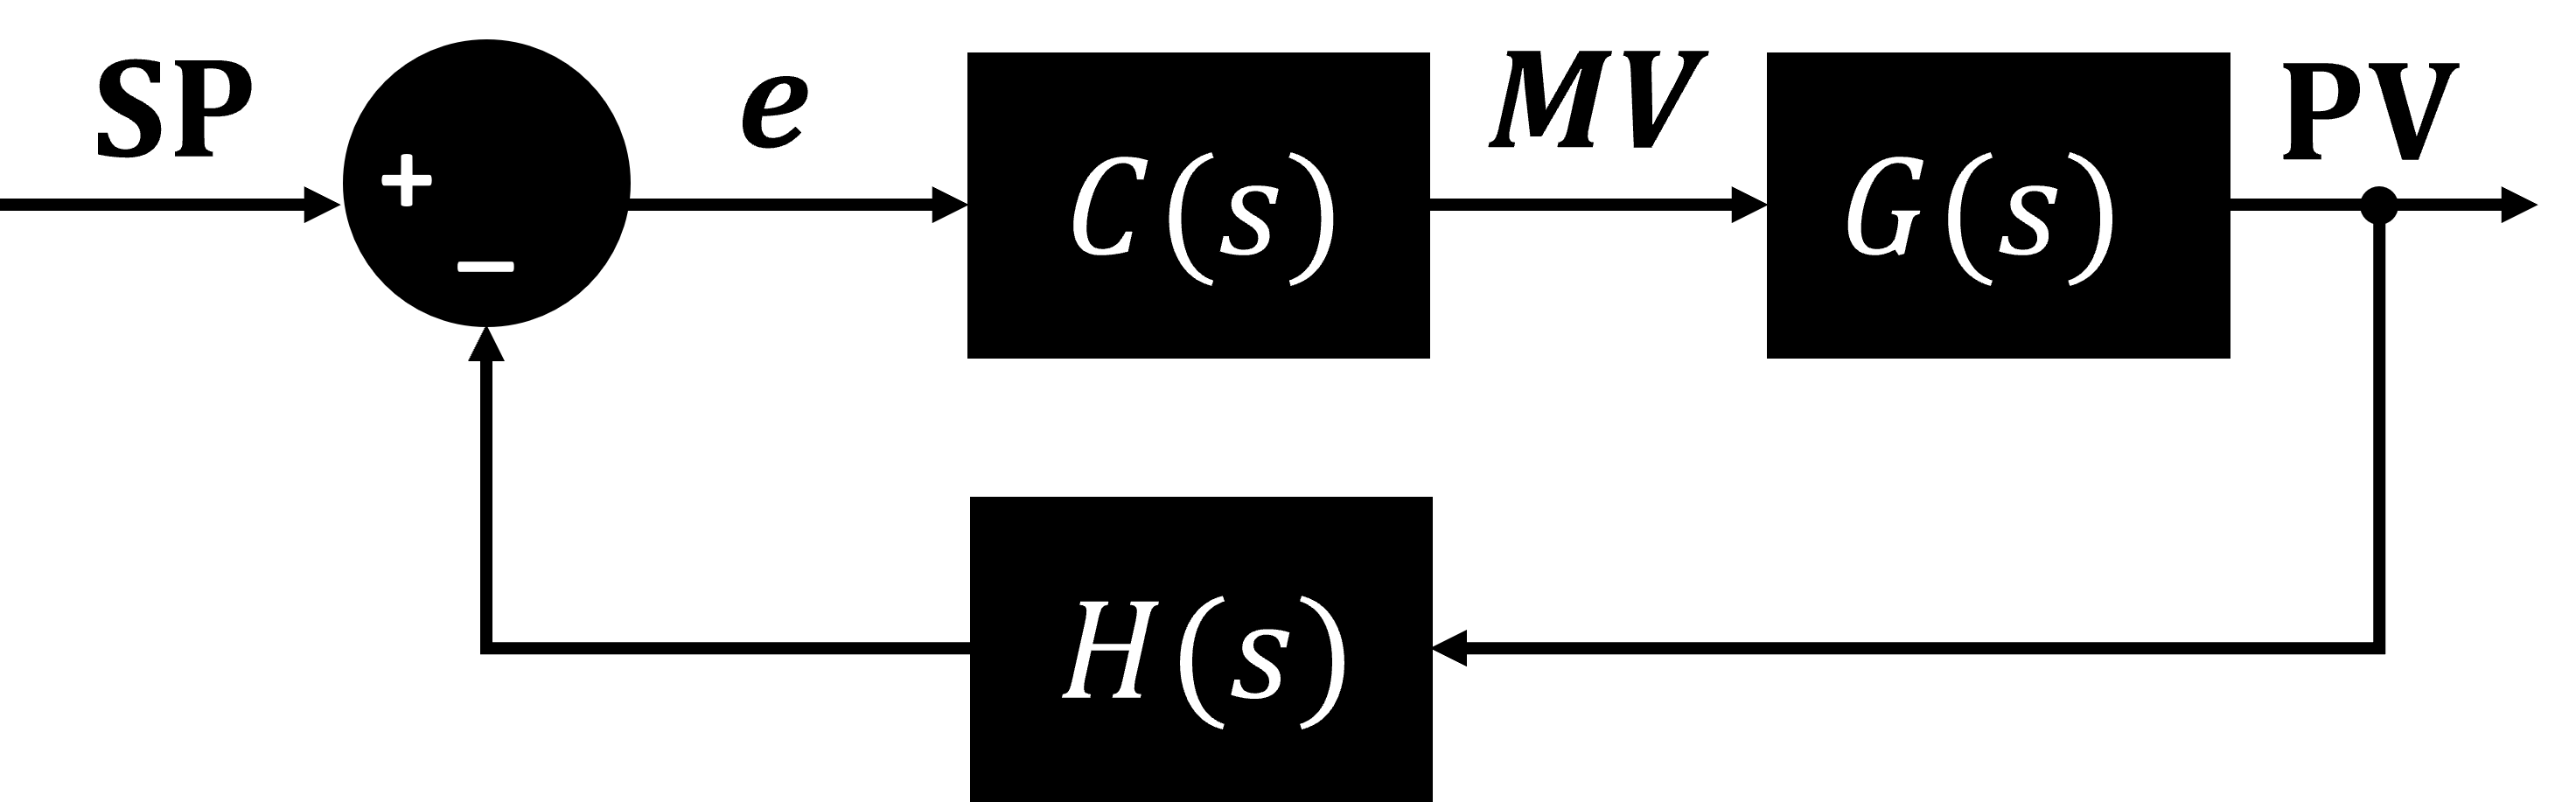
\includegraphics[width=0.48\textwidth]{Figuras/MalhaFechada.png}
                \caption{Sistema de controle em malha fechada.} \label{fig:MalhaFechada}
            \end{figure}
        \end{itemize}

        Apesar de caracterizar sistemas mais caros e de maior complexidade, na prática, os sistemas para controle de temperatura apresentam-se em malha fechada. Como vantagem, a malha de realimentação possibilita corrigir variações nos valores de saída em decorrência de pertubações que possam agir no sistema, além da mudança do \SetPoint.
    \subsection{Função de transferência}
        A função de transferência de um sistema de controle, no domínio da transformação de Laplace (variável \textit{s}), descreve a relação entre a saída e a entrada desse sistema, assumindo as condições iniciais nulas. 
        
        Uma função de transferência $H(s)$ pode ser representada pelos valores de $z_k$ (raízes do numerador ou zeros da função) e de $p_k$ (raízes do denominador ou polos da função). Considerando um sistema com $M$ zeros, $N$ polos e um fator de ganho $K$, o modelo é descrito pela Equação ~\ref{eq:FuncaoTransferencia}:
        \begin{equation}
            \label{eq:FuncaoTransferencia}
            H(s) = \dfrac{U(s)}{E(s)}= K \cdot \dfrac{\prod_{k = 1}^{M}(s - z_k)}{\prod_{k = 1}^{N}(s - p_k)}
        \end{equation}
        
        Analisando a função de transferência, os tipos de sistema são definidos de acordo com o número polos na origem $(s=0)$ existentes em malha aberta. A função é dita do tipo $n$ por possuir $n$ polos na origem. Os tipos de sistema possuem definições para o erro no regime permanente, elencados na Tabela ~\ref{tab:TabelaErros}, em que $K_p$, $K_v$ e $K_a$ são medidas dos erros para diferentes tipos de entrada:
        
        \begin{table}[H]
            \caption{Erro em regime permanente para os tipos de sistema.} \label{tab:TabelaErros}
            \centering
            \begin{tabular}{cccc} \cline{2-4}
                \rule{0mm}{3mm} & Degrau & Rampa & Parábola \\ \hline \vspace{0.1cm}
                \rule{0mm}{5mm} Tipo 0 & ${(1+K_p)}^{-1}$ & $\infty$  & $\infty$ \\ \hline \vspace{0.1cm}
                \rule{0mm}{5mm} Tipo 1 & 0 & ${K_v}^{-1}$ & $\infty$ \\ \hline \vspace{0.1cm}
                \rule{0mm}{5mm} Tipo 2 & 0 & 0 & ${K_a}^{-1}$ \\ \hline
            \end{tabular}
        \end{table}
        
        Além da classificação em tipos, os sistemas de controle são ditos de determinada ordem de acordo com o número de polos, $N$. Para sistemas com $N > 2$, os polos mais próximos ao eixo imaginário do plano \textit{s} apresentam uma resposta exponencial mais lenta e, dessa forma, determinam a dinâmica do sistema, sendo chamados de polos dominantes. Os polos mais distantes do eixo imaginário apresentam uma resposta exponencial mais rápida, não influenciando, intensamente, na análise da resposta temporal.
    \subsection{Sistemas de primeira ordem com tempo morto}
        Um sistema de controle de temperatura, geralmente, é modelado por uma função de transferência de primeira ordem com atraso de transporte (tempo morto), ou seja, um atraso na resposta do sistema. O modelo \textit{First Order Plus Dead Time (FOPDT)}, é descrito pela função de transferência da Equação ~\ref{eq:FOPDT}, em que \textit{k} é o ganho estático do sistema, $\tau$, a constante de tempo e $\theta$, o tempo morto, em segundos:
        \begin{equation}
            \label{eq:FOPDT}
            H(s) = \dfrac{k}{\tau s + 1} \cdot e^{-\theta s}
        \end{equation}
        
        O gráfico da Figura ~\ref{fig:GraficoAtraso}, compara as curvas da resposta de sistemas de primeira ordem com e sem tempo morto a uma entrada do tipo degrau. Na prática, o tempo morto pode representar o intervalo em que uma variação da grandeza de saída demora para ser detectada pelo elemento sensor, implicando em situações de acionamento ou desacionamento retardado do elemento atuador, levando a saída a um modo mais intenso de resposta. Nos casos em que o tempo morto é elevado, torna-se difícil obter um controle estável, pois o sistema tende a entrar em oscilação devido a essa condição \cite{ApostilaME}.  
        \begin{figure}[H]
            \centering
            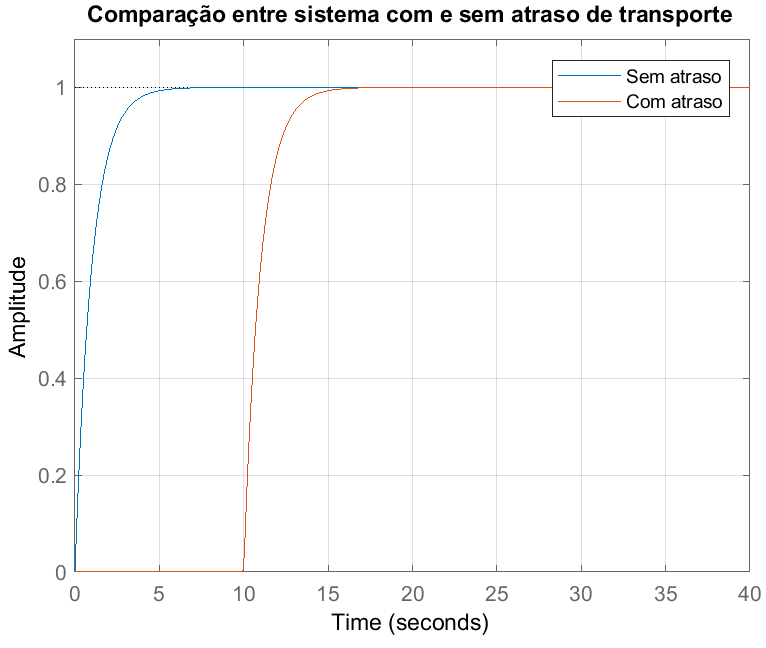
\includegraphics[width=0.45\textwidth]{Figuras/AtrasoTransporte.png}
            \caption{Comparação entre as curvas de sistemas com e sem tempo morto.} \label{fig:GraficoAtraso} 
        \end{figure}
    \subsection{Sistemas de segunda ordem}
        Os sistemas de segunda ordem em malha aberta são caracterizados por um modelo com dois polos, cuja função de transferência pode ser parametrizada segundo a Equação ~\ref{eq:SegundaOrdem}, em que $\xi$ representa o coeficiente de amortecimento do sistema e $\omega _n$, a frequência natural de oscilação:
        \begin{equation}
            \label{eq:SegundaOrdem}
            G(s) = \dfrac{\omega _n ^2}{s^2+2 \xi \omega _n \cdot s + \omega _n ^2}
        \end{equation}
        
        Para $0 < \xi < 1$, os polos em malha fechada são complexos e conjugados e estão presentes no semiplano esquerdo do plano \textit{s}, caracterizando um sistema sub-amortecido na resposta oscilatória. Com $\xi = 1$, a resposta oscilatória do sistema é criticamente amortecida, enquanto é superamortecida para $\xi > 1$.
        
        O gráfico da Figura ~\ref{fig:Resposta2Ordem}, ilustra a resposta genérica de um sistema de segunda ordem a uma entrada do tipo degrau, em que são denotados os seguintes parâmetros:
        \begin{figure}[H]
            \centering
            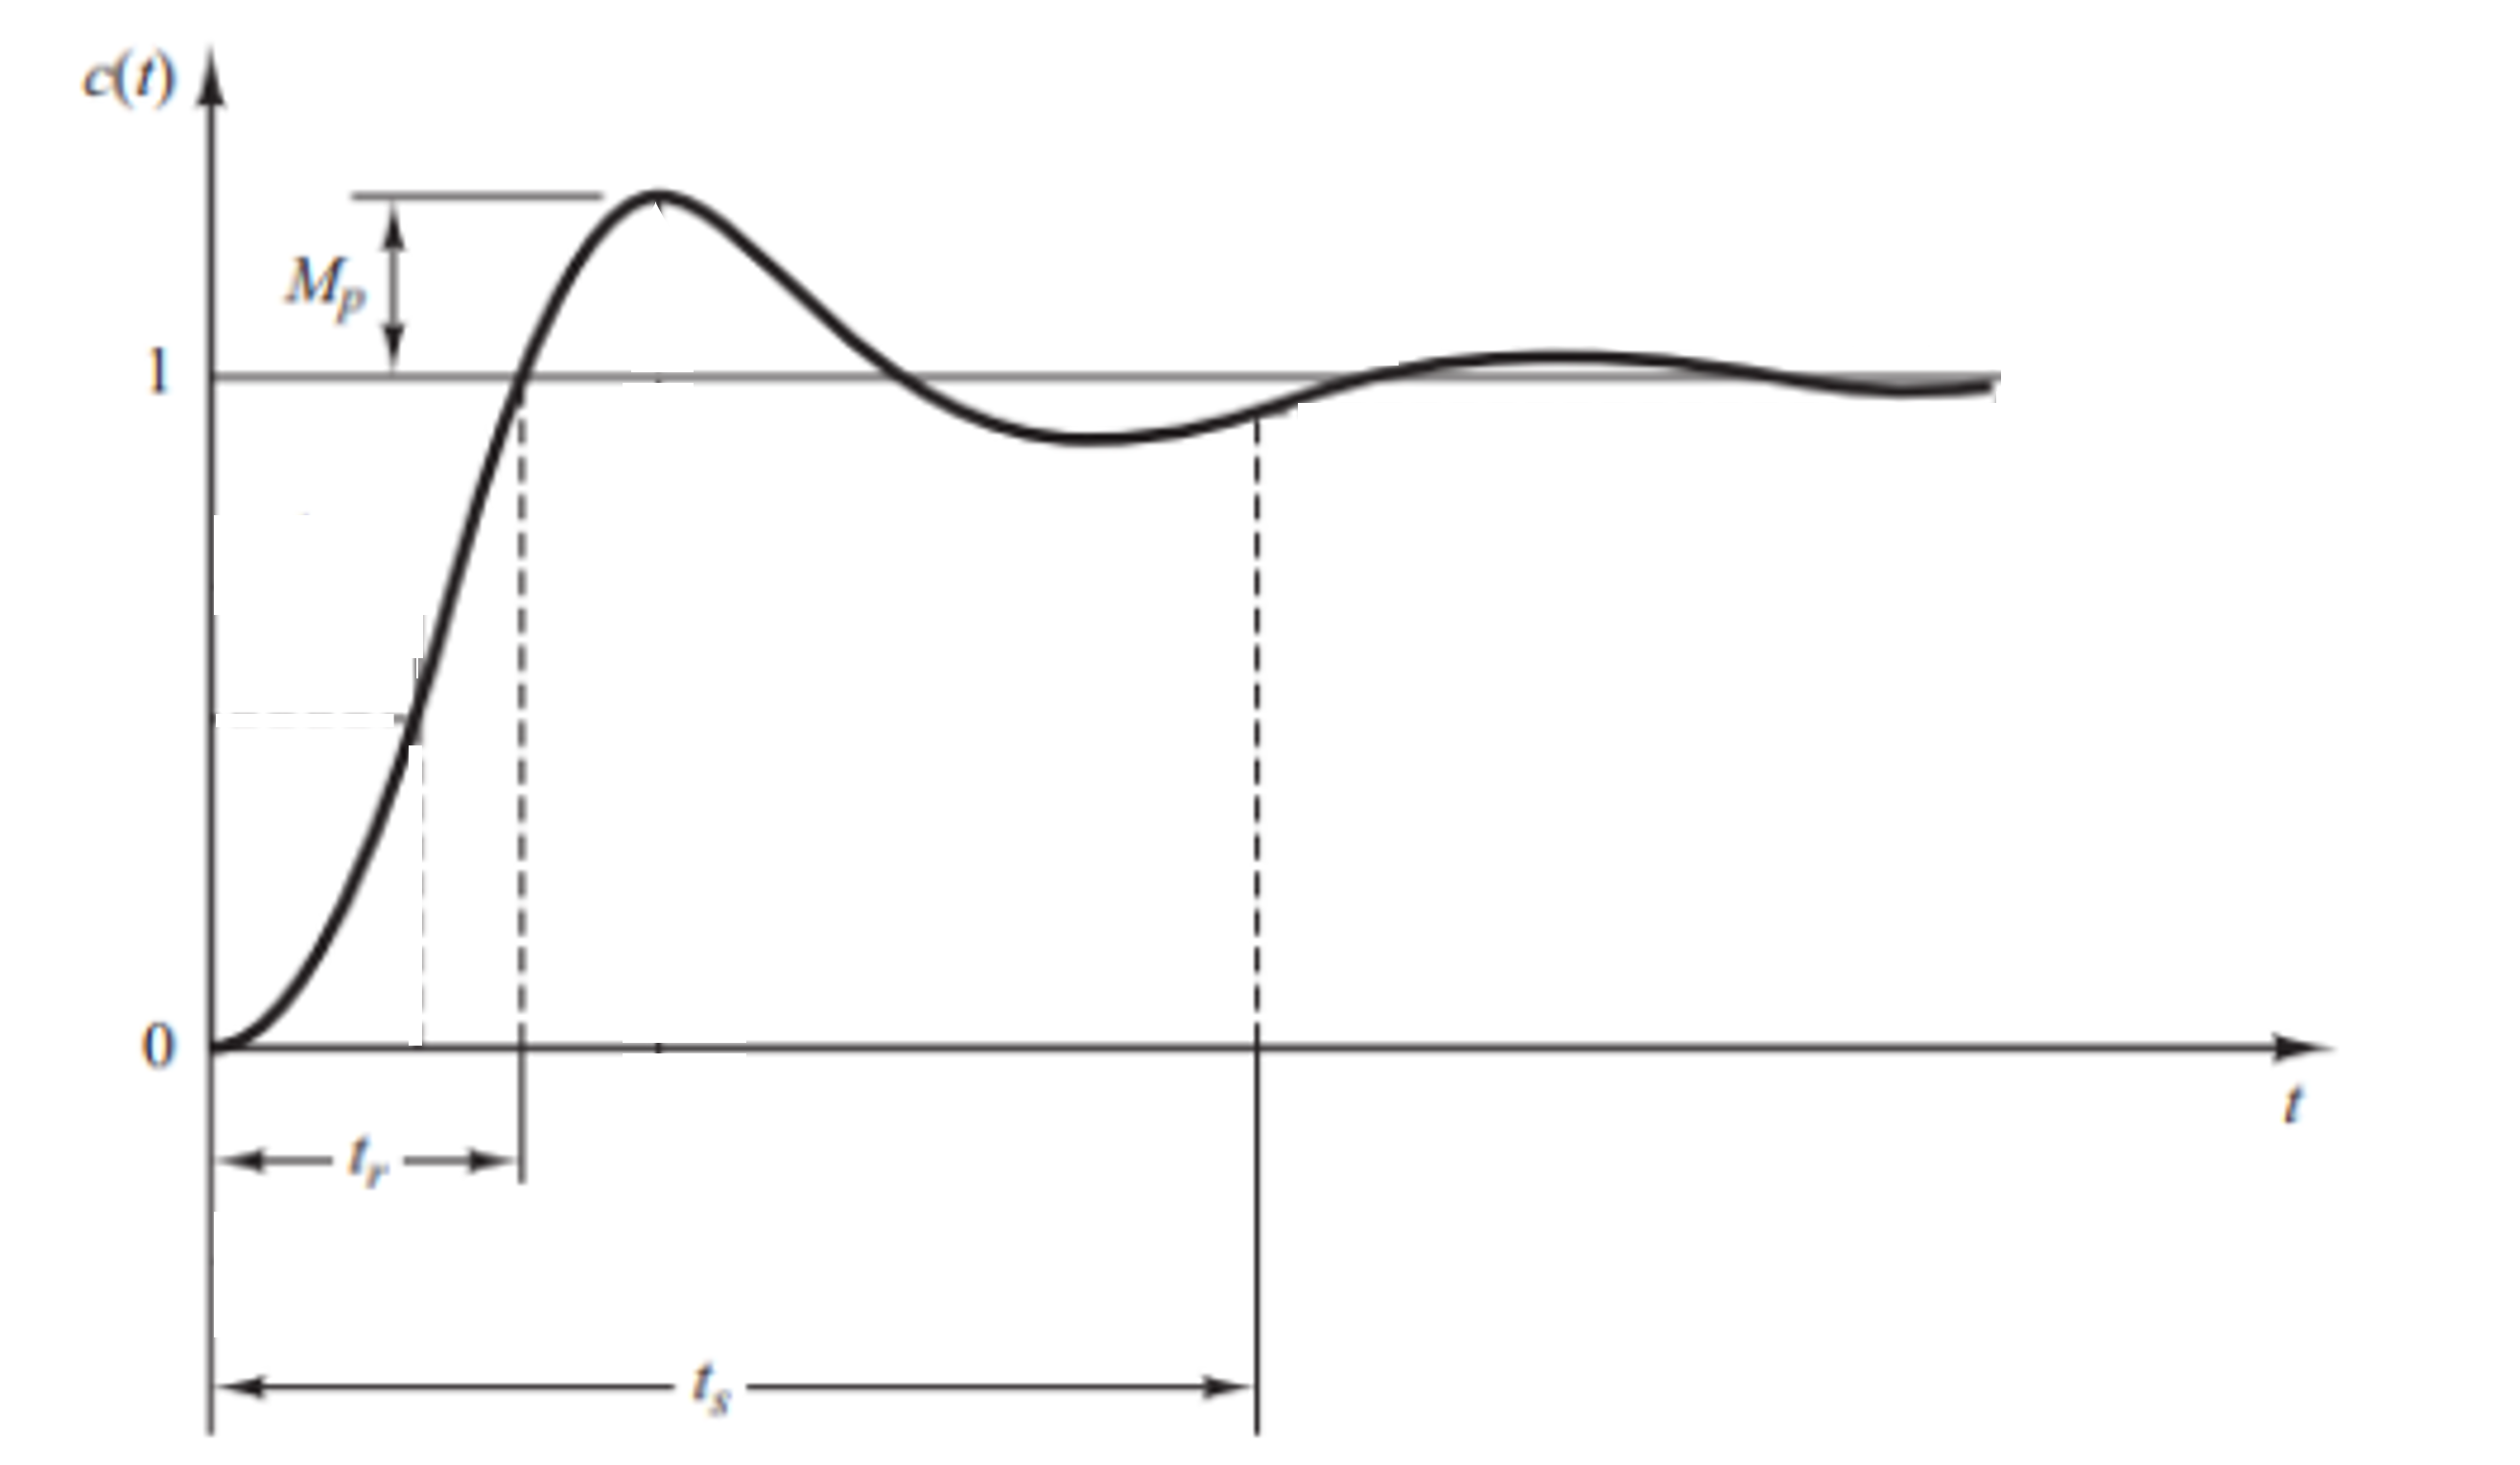
\includegraphics[width=0.48\textwidth]{Figuras/SegundaOrdem.png}
            \caption{Resposta típica de sistemas de segunda ordem.} \label{fig:Resposta2Ordem} 
        \end{figure}
        
        \begin{itemize}
            \item Tempo de subida $- \ t _r$: tempo para a curva de resposta passar de $10\%$ a $90\%$ (em sistemas superamortecidos) ou de $0\%$ a $100\%$ (em sistemas sub-amortecidos) do valor final;
            \item Tempo de acomodação $- \ t_s$: tempo do regime transitório do sistema, ou o tempo para entrar em regime permanente, normalmente com valores na faixa de $95\%$ a $98\%$ do valor final. É a maior constante de tempo do sistema de controle;
            \item Máximo pico (ou \textit{overshoot)} $- \ M_p$: representa o maior valor da curva de resposta do sistema, medido em porcentagem em relação ao valor final. Esse valor indica, diretamente, a estabilidade relativa do sistema.
        \end{itemize}
        
    O tempo de acomodação e o máximo pico do sistema são grandezas inversamente relacionadas, de forma que os sistemas mais rápidos, geralmente, apresentam valores mais elevados de \textit{overshoot}. Sistemas que devem possuir valores mais baixos (ou zerados) de máximo pico, por natureza, devem ser mais lentos.
        
    Em algumas técnicas, o modelo da função de transferência do sistema é do tipo $1$. Quando o controle é aplicado ao processo, a resposta típica se comporta como uma curva de segunda ordem, mesmo que o modelo tradicional do sistema, propriamente, não seja. Tal fato apresenta-se, por exemplo, no Controle PID, que, aplicado ao controle do forno de convecção forçada, resultará em uma resposta típica de segunda ordem.
